\newpage

\section{Plateau-Bereich}

Es werden zunächst folgende Daten gemessen:
\begin{table}
        \centering
        \caption{Messdaten zur Kennlinie}
        \begin{tabular}{c c}
            \toprule
            {Spannung U in $\si{\volt}$} & {Entladungen N in \text{imp/min}} \\
            \midrule
            320 & 	9672   \\
            330 & 	9689   \\
            340 & 	9580   \\
            350 & 	9837   \\
            360 & 	9886   \\
            370 & 	10041  \\
            380 & 	9996  \\
            390 & 	9943  \\
            400 & 	9995  \\
            410 & 	9980  \\
            420 & 	9986  \\
            430 & 	9960  \\
            440 & 	10219 \\
            450 & 	10264 \\
            460 & 	10174 \\
            470 & 	10035 \\
            480 & 	10350 \\
            490 & 	10290 \\
            500 & 	10151 \\
            510 & 	10110 \\
            520 & 	10255 \\
            530 & 	10151 \\
            540 & 	10351 \\
            550 & 	10184 \\
            560 & 	10137 \\
            570 & 	10186 \\
            580 & 	10171 \\
            590 & 	10171 \\
            600 & 	10253 \\
            610 & 	10368 \\
            620 & 	10365 \\
            630 & 	10224 \\
            640 & 	10338 \\
            650 & 	10493 \\
            660 & 	10467 \\
            670 & 	10640 \\
            680 & 	10939 \\
            690 & 	11159 \\
            700 & 	11547 \\
            \bottomrule 
        \end{tabular}
    \label{tab:a}
    \end{table}

    Der absolute Fehler für N Entladungen ergibt sich durch die Poissonverteilung zu:
    \begin{equation}
    \label{eqn:absoluterfehler}
    \Delta N = \sqrt{N}
    \end{equation}

    Die Werte werden mit Fehlern aus der Tabelle (\ref{tab:a}) in eine Grafik eingetragen und es es wird für das Plateau eine Ausgleichgerade modelliert. 
    \begin{figure}
	\centering
	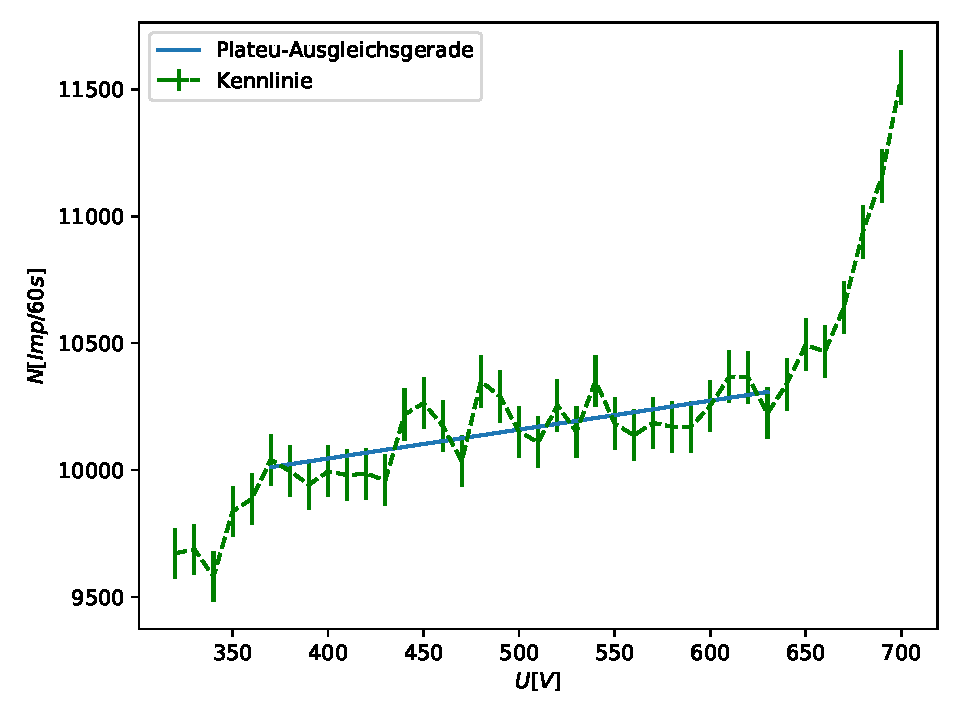
\includegraphics[width=0.8\linewidth]{Daten/a.pdf}
	\caption{Charakteristik des Zählrohres mit Fehlern und Plateaugerade.}
	\label{fig:plateau}
    \end{figure}

    Daraus ergibt sich für die Ausgleichgerade in der Form: 
    \begin{equation*}
    \label{eq:ausgleichsgerade}
    y = mx + b
    \end{equation*}

    \begin{align*}
    m &= 1.1377 \pm 0.2407\\
    b &= 9590.7346 \pm 121.8236.
    \end{align*}

    Daraus folgt dann das die Plateau-Steigung in $\si{\percent}$ pro $\SI{100}{\volt}$ gegeben ist durch:
    \begin{equation*}
    m = 1.1377 \pm 0.2407 \si{\percent} \text{pro 100V}.
    \end{equation*}





\section{Bestimmung der Totzeit}
    \subsection{Zwei-Quellen-Methode}
    Zur Bestimmung der Totzeit wurden die ermittelten Werte aus (\ref{n:n}) genutzt. Mithilfe der Formel (\ref{eqn:t}) und der Gauss Fehlerfortpflanzung welche gegeben ist durch:

    \begin{equation}
    \label{eqn:gauß}
    \sigma_T = \sqrt{ \left(\frac{N_{1+2}-N_{2}}{2N_{1}^{2}N_{2}}\right)^2 \cdot \sigma_{N_{1}}^2+ \left(\frac{N_{1+2}-N_{1}}{2N_{1}N_{2}^{2}}\right)^2 \cdot \sigma_{N_{2}}^2+\left(\frac{1}{2N_1N_2}\right)^2 \cdot \sigma_{N_{1+2}}^2} 
    \end{equation}

    Ergibt sich für die Totzeit folgender Wert:

    \begin{equation*}
    T = 0.00011 \pm 0.00005 \si{\second}.
    \end{equation*}



    \subsection{Oszilloskop}
    Mithilfe des Oszilloskops kann die Totzeit ebenfalls bestimmt werden. Die Methode ist jedoch sehr ungenau. Anhand des folgenden Bildes kann diese auf $T = 0.5 \pm 0.1 \si{\micro\second}$ 
    bestimmt werden. Die Zeitachse am Oszilloskop ist durch $100 \si{\micro\second}/DIV$ gegeben.
    \begin{figure}
	\centering
	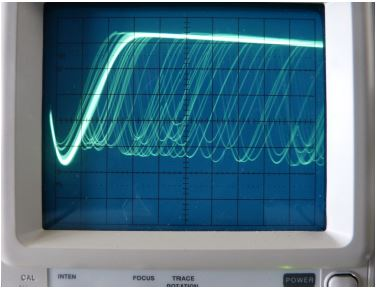
\includegraphics[width=0.8\linewidth]{Daten/c.JPG}
	\caption{Momentaufnahme eines Oszilloskops}
    \end{figure}

\section{Bestimmung des Zählrohrstroms}
    Aus dem mittleren Zählrohrstrom I kann die Zahl $Z = \frac{I}{\varepsilon_0 N} $ der freigesetzten Ladungen pro eingefallenen Teilchen berechnet werden. 
    Dazu wurden folgende Werte erhoben:

    \begin{table}
        \centering
        \caption{Zählerstrom Messdaten}
        \begin{tabular}{c c c}
            \toprule
            {Spannung U in $\si{\volt}$} & {Entladungen N in \text{imp/min}} & {Strom I in $\si{\micro\ampere}$}\\
            \midrule
            350 & 	          9837     &         0.3 \\
            400 &	          9995  &            0.4 \\
            450 &	          10264 &            0.7 \\
            500 &	          10151 &            0.8 \\
            550 &	          10184 &            1.0 \\
            600 &	          10253 &            1.3 \\
            650 &	          10493 &            1.4 \\
            700 &	          11547 &            1.8 \\
            \bottomrule 
        \end{tabular}
    \label{tab:c}
    \end{table}

    Mithilfe der Formel (\ref{eqn:i}) und $Z = \frac{I}{\varepsilon_0 N} $ kann der Zählerstrom berechnet und in eine Grafik eingetragen werden:
    \begin{table}
    \centering
    \caption{Errrechnete Daten}
    \begin{tabular}
    {S[table-format = 1.1] @{${}\pm{}$} S[table-format = 1.2]
     S[table-format = 2.4] @{${}\pm{}$} S[table-format = 1.4]
    }
    \toprule
    \multicolumn{2}{c}{$I \mathbin{/} \si{\micro\ampere}$}       &
    \multicolumn{2}{c}{$Z$ in Mrd.}                              \\
    \midrule
    0.3 & 0.05 & 11.4209 & 2.1021  \\
    0.4 & 0.05 & 14.9871 & 2.2041  \\
    0.7 & 0.05 & 25.5401 & 2.6722  \\
    0.8 & 0.05 & 29.5136 & 2.9242  \\
    1.0 & 0.05 & 36.7724 & 3.3686 \\
    1.3 & 0.05 & 47.4824 & 4.0656  \\
    1.4 & 0.05 & 49.9654 & 4.1785  \\
    1.8 & 0.05 & 58.3773 & 4.5097  \\
    \bottomrule
    \end{tabular}
    \end{table}

    \begin{figure}
	    \centering
	    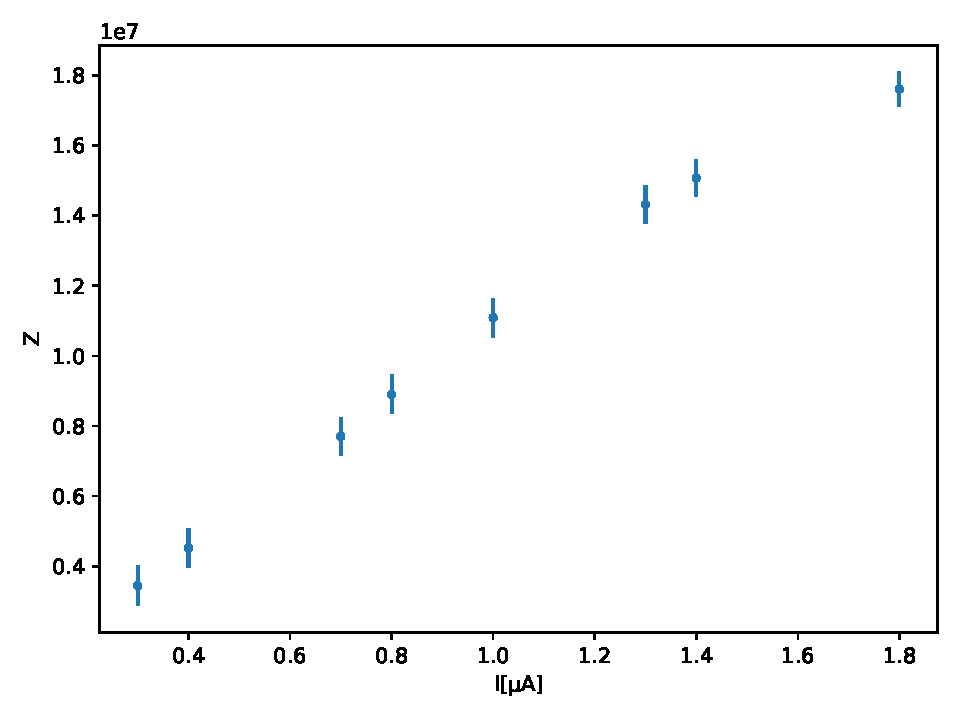
\includegraphics[width=0.8\linewidth]{Daten/d.pdf}
	    \caption{Errechneter Zählerstrom mit Fehler}
    \end{figure}